\chapter{Theoretical Background }\label{sec:theory}

\section{The learning framework}

Statistical learning theory encompasses the mathematical framework used to
study generalization in machine learning. In this formalism, the goal
is to learn a target function $f^*: \mathcal{X} \to \mathcal{Y}$ by means of an approximated
function $f \in \mathcal{F}$ using a finite set of observations. 

\begin{definition}[Supervised dataset]
    Let $\mathcal{X} \subseteq \mathbb{R}^d$ and $\mathcal{Y} \subseteq \mathbb{R}^t$ be
    the input and output spaces, respectively. Let $X$ be the random variable associated
    with the sampling in $\mathcal{X}$, and $\underbar{X} = (X_1, ..., X_N) \overset{\text{iid}}{\sim} X$ be a $N$-sized simple
    random sample of $X$. A supervised dataset $D$ is a realization of $\underbar{X}$ paired with its $f^*$-mapped output values.

    $$
    D = \{(\bm{x}_n, f^*(\bm{x}_n))\}_{n \in [N]}
    $$
\end{definition}

\subsection{Empirical risk minimization}

The quality of the approximation can be measured with the expected risk $\mathcal{R}(f)$

$$
\mathcal{R}(f)=\mathbb{E}_{x \sim X}[\mathcal{L}(f(x),f^\star(x))]
$$

where $\mathcal{L}: \mathcal{Y} \times \mathcal{Y} \to \mathbb{R}$ denotes a loss function. Glivenko-Cantelli theorem allow us to
estimate the expected risk with its empirical (plug-in) equivalent when $N$ is large enough.

\begin{definition}[Empirical risk] Let $D$ and $\mathcal{L}$ be the dataset and loss function of our problem, respectively. The empirical risk of $f \in \mathcal{F}$
    computed on $D$ is defined as

    $$
    \hat{\mathcal{R}}_D(f)=\frac{1}{N}\sum_{n=1}^{N}\mathcal{L}(f(\bm{x}_{n}),f^{\star}(\bm{x}_{n}))
    $$
\end{definition}

Training, therefore, amounts to minimizing the empirical risk over the function class $\mathcal{F}$.

$$
\text{ERM}_D = \hat{f}_D = \min_{f \in \mathcal{F}} \hat{\mathcal{R}}_D(f)
$$

The best learning algorithm will be that minimizing the difference between the 
expected and empirical risks computed on a different realization of the data. 

\begin{definition}[Empirical generalization error] Let $D_{t}$ and $D_v$ be two supervised datasets. Let $\hat{f}^* \in \mathcal{F}$ be the function minimizing the expected risk
    , and let $\hat{f}_{D_t}$ be the function minimizing the empirical expected risk computed on $D_t$. The empirical generalization error of $f_{D_t}$ computed on $D_v$ is defined as

    $$
    \mathcal{E}(D_t, D_v) = \hat{\mathcal{R}}_{D_v}(\hat{f}_{D_t}) = [\hat{\mathcal{R}}_{D_v}(\hat{f}) - \hat{\mathcal{R}}_{D_v}(\hat{f}^*)] + \hat{\mathcal{R}}_{D_v}(\hat{f}^*) = \mathcal{E}_{\text{estimation}}+ \mathcal{E}_{\text{capacity}}
    $$

    where $\mathcal{E}_{\text{capacity}}$ is governed by the ability of the function class $\mathcal{F}$ to represent the target function; i.e. its complexity.
\end{definition}


The definition of complexity depends on the problem, but intuitively measures the cardinality of the
subset of $\mathcal{F}$ that the algorithm is able to represent. A complex or high-capacity algorithm will
be able to represent a larger subset of $\mathcal{F}$ and achieve a low empirical error, but will be also
prone to overfitting to the specific learning realization thus yielding a higher generalization error. 

\subsection{Regularized risk minimization}

As a general principle, the inductive bias of the algorithm (i.e. the set of constraints imposed on $\mathcal{F}$ during learning) should be aligned with
that of our target function. Given that more expressive classes are always preferred by optimization algorithms, the ERM
objective function is usually tweaqued to include a regularization term penalizing complexity.

\begin{definition}[Regularized empirical risk] Let $\Omega: \mathcal{F} \to \mathbb{R}$ be a complexity measure. The regularized empirical risk of a function $f$
    computed on $D$ is defined as

    $$
    \hat{\mathcal{R}}_{\Omega}(f)=\hat{\mathcal{R}}(f) + \lambda \Omega(f)
    $$

    where $\lambda \in \mathbb{R}$ controls the trade-off between empirical risk and generalization error.

\end{definition}

The RRM problem now includes a hyperparameter $\lambda$, that will be selected so that the generalization error is minimized.

\section{Learning with neural networks}

Neural networks are biologically-inspired machine learning models that consist of a set of 
nodes (neurons) organized in layers and connected by weighted edges (synapses). Figure \ref{fig:nn_node} shows the 
data transformation performed by a single node.

\begin{figure}[H]
    \centering
    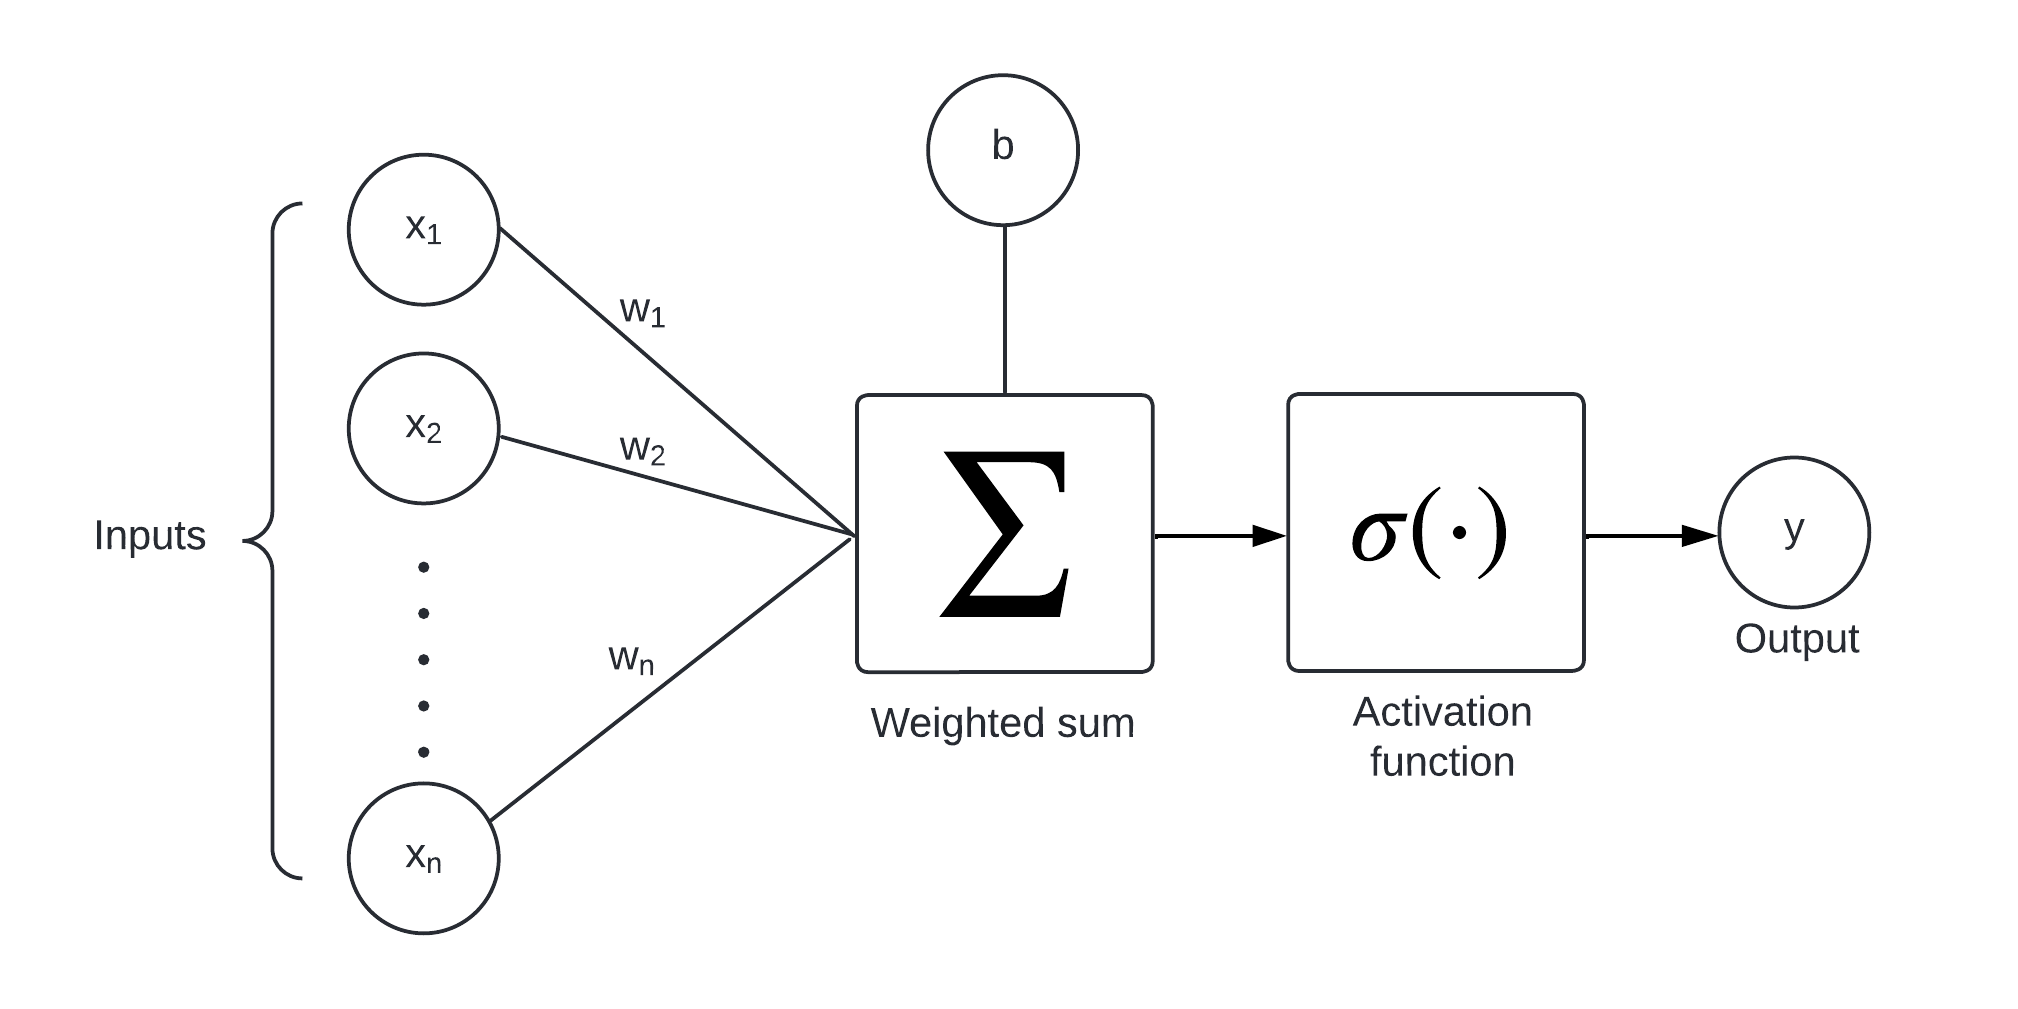
\includegraphics[width=0.4\textwidth]{img/theoretical_background/nn_node.png}
    \caption{The output of a node is computed by applying a non-linear
    activation function $\sigma(\cdot)$ to the weighted sum of its inputs.}
    \label{fig:nn_node}
\end{figure}

Let $\bm{x}_k \in \mathbb{R}^{d_k}$ be the input to the layer $k$, and let $\bm{W} \in \mathbb{R}^{d_k \times d_{k+1}}$ be the $k$-th weight matrix. The output of the layer can be expressed as

$$
\bm{x}_{k+1} = \sigma_k(\bm{z}_{k+1}) = \sigma_k(\bm{W}_k^T \bm{x}_k + \bm{b}_k)
$$

where $\sigma_k$ is the non-linear activation function at layer $k$. We can therefore express the overall transformation of a neural network
as the composition of its layers.

$$
f_{\text{NN}}(\bm{x}) = \bigcirc_{k=0}^{L-1} \sigma_k(\bm{W}_k^T \bm{x} + \bm{b}_k) = f(\bm{x}; \bm{\gamma})
$$

where $\bm{\gamma}$ represents the set of parameters of the network. In order to solve the learning problem, the optimization algorithm must navigate the non-convex loss
landscape towards the minimum of the empirical risk. This is computationally achieved by means of gradient-descent-based algorithms, which compute the
gradient over the parameters by means of the backpropagation algorithm.

\subsection{Backpropagation and gradient descent}

Let $w_{ji}^{(k)}$ be the weight from node $j$ on layer $k-1$ to node $i$ on layer $k$. Let $a_i^{(k-1)}$ be the output of node $i$ on layer $k-1$ and let $z_j^{(k)} = \sum_{i=0}^{n_k - 1} w_{ji}^{(k)} a_i^{(k-1)} + b_k^{(k)}$ be 
the linear input of node $j$ on layer $k$, so that $a_j^{(k)} = \sigma_j(z_j^{(k)})$ is the ouput from node $j$. We can compute the gradient of the loss $\mathcal{L}$ with respect to the weights by means of the chain rule as follows: 

$$  
\frac{\partial \mathcal{L}}{\partial w_{ji}^{(k)}} = \frac{\partial \mathcal{L}}{\partial a_{j}^{(k)}} \frac{\partial a_{j}^{(k)}}{\partial z_{j}^{(k)}} \frac {\partial z_{j}^{(k)}} {\partial w_{ji}^{(k)}} =
\frac{\partial \mathcal{L}}{\partial a_{j}^{(k)}} \frac{\partial \sigma_j^{(k)}}{\partial z_{j}^{(k)}} a_i^{(k-1)}
$$

Given that the loss is computed as a function of the output of the network, all the edges from node $i$ of layer $k-1$ influence the loss value at that node:

$$
\frac{\partial \mathcal{L}}{\partial a_{i}^{(k-1)}} = \sum_{j=0}^{n_{k} - 1} \frac{\partial \mathcal{L}}{\partial a_{j}^{(k)}}  \frac{\partial a_{j}^{(k)}}{\partial z_{j}^{(k)}} \frac{\partial z_{j}^{(k)}}{\partial a_{i}^{(k-1)}} =
\sum_{j=0}^{n_{k} - 1} \frac{\partial \mathcal{L}}{\partial a_{j}^{(k)}} \frac{\partial \sigma_j^{(k)}}{\partial z_{j}^{(k)}} w_{ji}^{(k)}
$$

All in all, we see that the same terms are required in different nodes to compute the gradient, making backpropagation algorithm very efficient. Equivalently, for the bias term:

$$
\frac{\partial \mathcal{L}}{\partial b_{j}^{(k)}} = \frac{\partial \mathcal{L}}{\partial a_{j}^{(k)}} \frac{\partial a_{j}^{(k)}}{\partial z_{j}^{(k)}} \frac {\partial z_{j}^{(k)}} {\partial b_{j}^{(k)}} = \frac{\partial \mathcal{L}}{\partial a_{j}^{(k)}} \frac{\partial \sigma_j^{(k)}}{\partial z_{j}^{(k)}}
$$

These derivatives are the components of the gradient vector that will be used to update the weights and biases of the network.

$$
w_{ji}^{(k)} = w_{ji}^{(k)} -\eta \frac{\partial \mathcal{L}}{\partial w_{ji}^{(k)}}
$$

$$
b_{j}^{(k)} = b_{j}^{(k)} -\eta \frac{\partial \mathcal{L}}{\partial b_{j}^{(k)}}
$$

where $\eta$ is the learning rate. More efficient variations of gradient descent such as stochastic gradient descent or Adam are used in practice.


\subsection{Loss landscape and parameter space}


A neural network architecture $\text{NN}$ can be expressed as a parametrization of the function space $\mathcal{F}$.

$$
    \begin{aligned}
        \text{NN}: \bm{\Gamma} & \subseteq \mathbb{R}^{S} \longmapsto \mathcal{F}_{\bm{\Gamma}} \\
        \bm{\gamma} & \longmapsto f(\bm{x}; \bm{\gamma}) = f_{\text{NN}}(\bm{x})
    \end{aligned}
$$

where $\Gamma$ is the parameter space associated with this particular architecture. The functional
landscape $\mathcal{F}_{\bm{\Gamma}}$ consists of all mappings $f(\bm{\gamma}): \mathcal{X} \longmapsto \mathcal{Y}$ that 
that can be realized by some parameter configuration $\bm{\gamma} \in \bm{\Gamma}$. \\

Universal approximation theorems state that arbitrarily wide or abitrarily deep architectures
are able to represent virtually any function, but it is an open challenge to theoretically describe which
complexity measure regulates generalization. A possible approach to this problem is to
study the geometry of the loss landscape, especially in the vicinity of local minima. For instance, 
connected flat minima are often linked to better generalization capabilities, as they
intuitively represent a robust manifold in the parametrization space and should be preferred over sharp minima. \\

In this work we will explore a different approach to the generalization problem, based on
a definition of the generalization error that relies on the implicit randomness of the
data sampling process. 

\section{Generalization error}

As we mentioned in the first lines of this chapter, the input of learning algorithms are
realizations of the random variable $X$ defined over the input space $\mathcal{X}$. The
implicit randomness embedded in the sampling process extends to the outcome of algorithms,
even when performing a deterministic sequence of operations. An alternative intuition of 
generalization arises from this perspective, in the sense that a learning algorithm should
learn the same function $f$ when trained on different realizations of the same experiment. This
intuition will be formalized in this section.\\

\subsection{Posterior distribution}

The function $f \in \mathcal{F}$ was defined mapping $\mathcal{X} \longmapsto \mathcal{Y}$, in the sense that an observation $x \in \mathcal{X}$ is mapped to
a prediction $f(x) \in \mathcal{Y}$. In order to formalize the randomness of the data sampling process, we
will redefine $\mathcal{X}$ so that its elements are realizations of the simple 
random sample $\underbar{X}$, which are then mapped to a set of outcomes $\theta$.

\begin{definition}[Distribution of $\underbar{X}$]
    The simple random sample $\underbar{X} \overset{\text{iid}}{\sim} X$ has a probability distribution
    described by the density function $f_{\underbar{X}}$.

    $$
     f_{\underbar{X}} = \prod_{n=1}^{N} f_{X}(x)
    $$

    We will refer to this probability distribution as $\mathbf{P}_X$ to avoid notation clutter.
\end{definition}

\begin{definition}[Hypothesis class]
    A data science algorithm learns a function $f$ implementing the following mapping:

    $$
    \begin{aligned}
        f: \mathcal{X} & \longmapsto \Theta \\
        \bm{x} = (x_1, \dots, x_N) \sim X  & \longmapsto (f(x_1), \dots, f(x_N)) = \theta
    \end{aligned}
    $$

    The output space of hypothesis $\Theta$ represents all possible outcomes of a function
    $f$ learned on a dataset sampled from $\mathcal{X}$.

\end{definition}

Intuitively, this framework interprets complexity from the perspective of the possible
set of outcomes of the function, rather than the function class itself. It can be argued
that both perspectives are equivalent, in the sense that the function class can be mapped 
to the hypothesis space $\Theta$. Nevertheless, more suitable generalization regularization
constraints can be defined in $\Theta$, especially when dealing with intractable
function classes $\mathcal{F}_{\Gamma}$ derived from deep neural networks. \\

For instance, complexity in the hypothesis class can be associated to the nature of the
randomness displayed by $X$. Ideally, too restrictive hypothesis classes that lack desirable
hypothesis for some realization $\bm{x}$ of $\underbar{X}$ should be avoided, and also those hypothesis
classes containing unrealizable elements (i.e. hypothesis that are not outcome of
any possible experiment). A richness condition can thus be postulated following
this intuition. \\

\begin{definition}[Richness condition]
    Let $\tau \in \mathbb{T}$ be a transformation of the sampling experiment $X$. The dependency
    of the data on the experimental design will be captured by the index $\tau$, and we will
    implicitely consider $\underbar{X}$ to be a sample of $\tau \circ X$.  We require a
    sufficiently rich set of experiments $\mathbb{T}$ such that every hypothesis $\theta \in \Theta$
    is the (most likely) outcome of some realization $\bm{x}$.

    $$
    \forall \theta, \exists \tau \in \mathbb{T} \text{ such that } f(\bm{x}) = \theta
    $$
\end{definition}


Since we assume a mapping $f$ and a data distribution $\mathbf{P}_X$, we can describe
the randomness of the hypothesis outcome conditioned on the the distribution of the data.

\begin{definition}[Posterior]
    A probability distribution over the hypothesis class can be defined as a 
    conditional distribution given an realization $\bm{x}$ of experiment $\underbar{X} \sim \mathbf{P}_X$. We will
    refer to this distribution as the posterior over $\Theta$ under $f$.

    $$
        \begin{aligned}
            f: \mathcal{X} \times \Theta & \longmapsto \mathbb{R} \\
            (\bm{x}, \theta) & \longmapsto \mathbf{P}^f (\theta \mid \bm{x})
        \end{aligned}
    $$

    $\mathbf{P}^f$ establishes the stochastic relation between data and hypothesis.
    
\end{definition}

Using these definitions we can operate over $\Theta$ within the framework of probability 
theory. For instance, we can obtain the (prior) probability of a hypothesis to be
selected by $f$ given $\underbar{X}$ as

$$
 \Pi^f (\theta) = \mathbb{E}_X \mathbf{P}^f (\theta \mid \bm{x})
$$

from which we can derive a probabilistic version of the richness condition, where a limit
case can be imposed with exactly one experiment per hypothesis, leading to a uniform prior:

$$
\Pi^f (\theta) = |\Theta|^{-1}
$$

Within this framework, selecting suitable hypothesis classes amounts to selecting
posterior distributions that yield a higher probability to the desired subset of hypothesis. This
is the leading principle that will guide the derivations that follow.

\subsection{Generalization error}

In order to define a generalization error within this framework, we will proceed in an
analogous way as we did in the previuous section. We will consider two datasets $D_t$ and $D_v$
that arise from two different sampling realizations. In this case, however, we will make
explicit the fact that they encode different instantiations of the randomness associated
with the sampling, and thus denote $\bm{x'}$ and $\bm{x''}$ as realizations of the two simple random
samples $\underbar{X}', \underbar{X}'' \overset{\text{iid}}{\sim} X \mid \tau$, respectively, and associate
each dataset with one of them. The $\tau$ indexing is now explicit, since both samples are conditionally
independent given the experiment:

$$
    \mathbf{P}(\underbar{X}', \underbar{X}'') = \mathbf{P}(\underbar{X}' \mid \tau) \mathbf{P}(\underbar{X}'' \mid \tau)
$$

The selection principles for a posterior distribution will be the following:
\vspace{-2mm}
\begin{description}
    \item[P1] It should be expressive enough to cover the realizable $\Theta$.
    \vspace{-3mm}
    \item[P2] Equally likely inputs drawn from the same experiment should yield similar sets of hypothesis.
\end{description}

\begin{definition}[Description length]
    Let $\mathcal{F}_{\bm{\Gamma}}(\cdot)$ be the function class containing all functions 
    represented by the parametrization $\bm{\Gamma}$. Let $\mathbf{P}_{\bm{\Gamma}}$ be the
    universal distribution relative to $\mathcal{F}_{\bm{\Gamma}}$ fulfilling the minimum
    description length principle. The description length of a function $f_\gamma \in \mathcal{F}_{\bm{\Gamma}}$ 
    is defined as the number of bits required to encode its parameters. The code length
    of the argument of such distribution is

    $$
    \text{DL}_{f_{\gamma}}(\cdot) = -\log f_{\gamma}(\cdot)
    $$
\end{definition}

The quality of the represented function $f$ will be measured by the description
length of its posterior, and thus a loss function can be defined as follows.

$$
    \ell (\theta, \bm{x}) = - \log \mathbf{P}^f (\theta \mid \bm {x})
$$



Given that the description length encompasses also the complexity of the hypothesis
class and not only the generalization capabilities, we will normalize the loss dividing by the
description length of the prior.

$$
    - \log \Pi^f (\theta) = - \log \mathbb{E}_X \mathbf{P}^f (\theta \mid \bm{x})
$$

\begin{definition}[Generalization error]
    Let $\bm{x'}$ and $\bm{x''}$ be realizations of $\underbar{X}', \underbar{X}''$, respectively.
    Let $\Theta$ be the hypothesis class represented by $f$ given data $X$. The generalization error 
    in the support $\mathcal{X}$ is defined as the out-of-sample description length:

    $$
        \mathcal{G}_{\mathcal{X}} = \mathbb{E}_{X', X''} \mathbb{E}_{\theta \mid X'} \left[ - \log \frac{\mathbf{P}^f(\theta | \bm{x}'')}{\Pi^f (\theta)} \right]
    $$
    
\end{definition}



It amounts to the expected normalized loss over the validation data $\bm{x}''$ computed
over the distribution on the hypothesis expressed by the posterior on the training data $\bm{x}'$.
Intuitively, a lower generalization error is achieved when good quality posteriors on $\bm{x}''$ are 
assigned a high probability by the posterior on $\bm{x}'$. 

\begin{lemma}[Posterior agreement]
    The generalization error $\mathcal{G}_{\mathcal{X}}$ is non-negative and has a lower bound $-\mathcal{J}$. We define $\mathcal{J}$ as the posterior agreement.
\end{lemma}
\begin{proof}
    $$
    \begin{aligned}
        \mathcal{G}_{\mathcal{X}} & \geq \mathbb{E}_{X', X''}\left[-\log \left(\mathbb{E}_{\theta \mid X'} \frac{\mathbf{P}^{f}\left(\theta \mid \bm{x}''\right)}{\Pi^{f}(\theta)}\right)\right] \\
        & =\mathbb{E}_{X', X''} \left[-\log \left(\sum_{\theta \in \Theta} \frac{\mathbf{P}^{f}\left(\theta \mid \bm{x}'\right) \mathbf{P}^{f}\left(\theta \mid \bm{x}'' \right)}{\Pi^{f}(\theta)}\right)\right] = -\mathcal{J} \\
        & \geq-\log \left(\mathbb{E}_{X', X''} \mathbb{E}_{\theta \mid X'} \mathbb{E}_{\theta \mid X''} \frac{\mathbf{P}^{f}\left(\theta \mid \bm{x}''\right)}{\Pi^{f}(\theta)}\right)=0 .
    \end{aligned}
    $$
\end{proof}

where Jensen's inequality has been applied twice to the convex function $-\log(\cdot)$:

$$
    \log (\mathbb{E} [\cdot]) \leq \mathbb{E}[\log( \cdot)]
$$

\subsection{Maximum posterior agreement}

Describe max posterior agreeement problem. All Joachim, but be brief.

\section{Posterior agreement kernel}

\subsection{Classification problem}

Statement of the classification problem. Follow structure from 


\section{DS algorithms, NNs and distribution shift}
MOST COMPLICATED SECTION. \\
- Cite Joachim, introduction to DS algorithms. Introduce notation that will follow the
rest of the thesis. Particularize for NNs (work to do).\\
- Explain function representation problem in NNs, why it is important. (look at phd zotero) \\
- Read about info theory, why description length  \\
- Start with two datasets, training and validation, and their distributions (also Joachim) \\
- Derive the OOD-error from the previous theory. More detail than Joachim. \\

\section{From OOD error to PA}
- Definitions and proofs (ommitted by Joachim) that lead to PA \\
- Intuition behind PA, plot. \\
- Read more about previous work from Joachim, where PA has worked. \\
- Include (briefly) the binary symmetric channel as an example, as it is 
important for Joachim and will be referenced later. \\

\section{The PA kernel}
- Follow derivation overleaf, include factorization theorem. \\
- Explain change of perspective, think of (binary) classification as a binary
symmetric channel. \\

\subsection{Properties}
(all in overleaf or papers) \\
- Positive definiteness, explain why important \\
- Symmetry, explain why important \\
- Convexity analysis. \\
- Problem with binary classification \\

\subsection{Example}
- Analytical results obtained, overleaf. \\


\section{Generalization error in the hypothesis space}
- Alternative formulation \\
- Explain why important, and formalize the data augmentation strategy (presentation) \\

